\chapter{A ligação química Carbono-Carbono}
\begin{mdframed}[backgroundcolor=orange!20,linewidth=0pt,roundcorner=10pt]
	\minitoc
\end{mdframed}
Sabemos que um átomo é formado, de modo simplista, por duas regiões distintas em termos de tipo de partícula e também de densidade de partículas: o núcleo do átomo de carbono é bastante denso em termos de partículas e a chamada eletrosfera é rarefeita em quantidade de partículas.

A conexão que átomos fazem entre si ocorre na eletrosfera chama-se \textbf{ligação química}. Precisamos compreender, inicialmente, como os elétrons ficam dispostos nessa região e também o que é necessário para que esses elétrons mantenham-se próximos a outros elétrons que estão localizados em outros átomos.

As propostas de organização da eletrosfera atômica iniciaram-se com as revolucionárias ideias de \textbf{Ernest Rutherford}, como resultado dos experimentos da espalhamento de partículas alfa, realizados no icônico Laboratório Cavendish \footnote{Veja aqui o site do Laboratório Cavendish: https://www.phy.cam.ac.uk/}, na Universidade de Cambridge, no Reino Unido. Embora fossem revolucionárias, as ideias de Rutherford sobre a eletrosfera eram incompatíveis com conceitos sólidos a respeito de Eletromagnetismo.

Torna-se necessário analisar como ocorre a conexão entre dois átomos por meio de orbitais atômicos e, sabendo que elétrons ficam em orbitais, é importante que saibamos como se dará a aproximação e como ficam esses orbitais após a conexão entre os dois átomos. Torna-se necessário agora entender rapidamente o modelo atômico apoiado em conceitos da Mecânica Quântica.

Atualmente, a eletrosfera do átomo é organizada em níveis de energia, subníveis e, finalmente, \textbf{orbitais} \index{orbitais}, onde localizam-se os elétrons. Tecnicamente e de acordo com a IUPAC, \textbf{orbital é a função de onda monoeletrônica obtida pela solução da Equação de Schrödinger para um átomo \footnote{O tratamento matemático necessário para plena compreensão deste assunto está além do escopo deste livro e sugerimos a consulta a textos especializados em Mecânica Quântica.}}. A Figura \ref{fig:orbitais} mostra um quadro bem interessante a respeito de orbitais.

\begin{figure}[h]
\centering
\vspace{0.25cm}
\caption{Subníveis dos tipos \textbf{s}, \textbf{p}, \textbf{d} e \textbf{f}, com seus respectivos orbitais.}
\label{fig:orbitais}
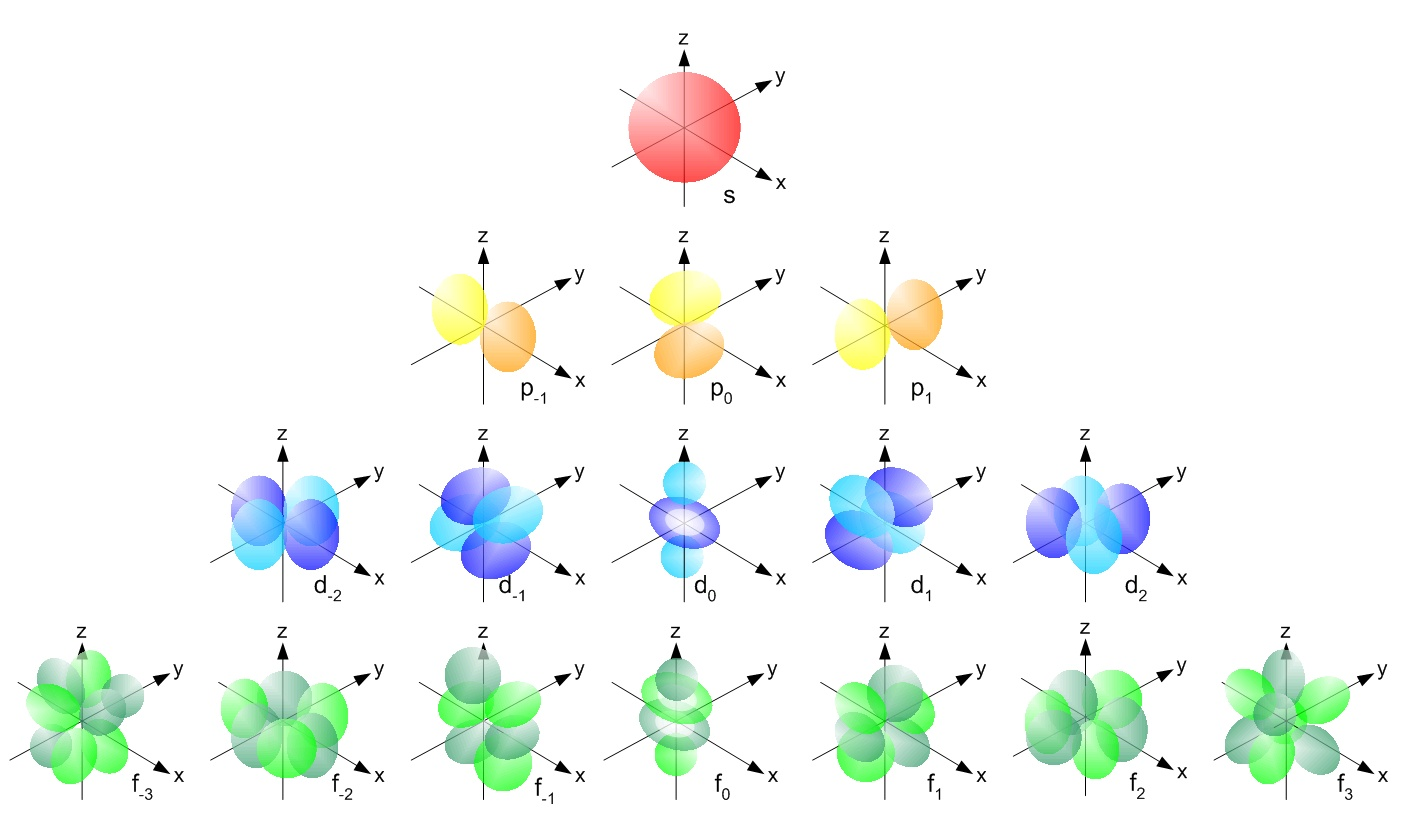
\includegraphics[width=1\linewidth]{imagens/all_orbitals.jpg}
\caption*{Fonte: Wikipedia, disponível em https://shorturl.at/eNY27}
\end{figure}

Cada parte colorida da Figura \ref{fig:orbitais} indica as regiões onde elétrons podem ser encontrados. O subnível s, que aparece na primeira linha da figura, é formado por apenas um orbital de forma esférica e os dois elétrons que esse orbital pode acomodar (assim como todos os demais orbitais) podem ocupar qualquer posição dentro da esfera. Uma evolução às ideias de Bohr, considerando a eletrosfera era unidimensional, as formas refletem a construção do modelo a partir das contribuições de Erwin Schrödinger e suas funções de onda, permitindo ao elétron ocupar determinadas regiões no espaço, mapeadas por coordenadas espaciais, chamadas de \textbf{números quânticos}. A segunda linha da figura apresenta o chamado subnível p, composto por três orbitais orientados em um sistema tridimensional e cada orbital é indicado de acordo com o eixo de orientação no qual se encontra: px, py e pz. Vale o mesmo raciocínio para os demais orbitais, mas nosso foco será no carbono.

\section{Números quânticos}
Conceitualmente e de modo simplificado, os números quânticos conhecidos por \textbf{principal}, \textbf{angular} e \textbf{magnético} definem, respectivamente, o tamanho, o formato e a orientação de cada orbital no espaço. 

O número quântico principal, representado pela letra \textbf{n} define o tamanho do orbital e está relacionado diretamente com o conceito anterior de \textbf{camada eletrônica}. Na Classificação Periódica dos Elementos (CPE) podemos observar a existência de sete períodos (ou linhas horizontais), diretamente relacionados com os sete níveis de energia conhecidos atualmente. Assim, um elemento presente no quinto período da CPE utiliza 5 níveis de energia para distribuir seus elétrons. O modo como tais elétrons são distribuídos em subníveis será visto mais adiante.

O formato do orbital é determinado pelo número quântico \textbf{angular} (chamado em alguns textos por secundário), representado pela letra \textbf{l} e está relacionado com o novo conceito de \textbf{subníveis}, ou cada uma das divisões de um dado nível de energia. Cabe aqui um esclarecimento muito importante: \textbf{subníveis são conjuntos de orbitais}. São utilizados atualmente, para os elementos conhecidos, quatro subníveis distintos e identificados pelas letras \textbf{s} (sharp, l = 0), \textbf{p} (principal, l = 1), \textbf{d} (diffuse, l = 2) e \textbf{f} (fundamental, l = 3).

Cada subnível também pode ser identificados por números e o número de orbitais em cada subnível é determinado por uma equação simples:

\begin{equation}
    m = 2\cdot l+1
    \label{eqn:orbitais}
\end{equation}

A equação \ref{eqn:orbitais} introduz o terceiro número quântico \textbf{m}, chamado de \textbf{magnético} e indica a orientação espacial de cada orbital em um dado subnível. Deste modo, quando falamos de um elétron localizado no quarto nível de energia (n = 4) e com número quântico angular com valor 2 (l = 2), temos possíveis 5 orbitais e, naturalmente, o mesmo número de orientações espaciais, e os valores numéricos que indicam esses orbitais estão na faixa (-l, ..., 0, ..., +l), com aplicação da equação \ref{eqn:orbitais}.

Aplicando essas ideias na análise da Figura \ref{eqn:orbitais}, entendemos o motivo pelo qual temos apenas \textbf{um} orbital no subnível s, \textbf{três} orbitais no subnível p, \textbf{cinco} orbitais no subnível d e \textbf{sete} orbitais no subnível f.

O chamado \textbf{Princípio da Exclusão de Pauli} \cite{massimi2005pauli} estabelece que dois elétrons não podem apresentar o mesmo conjunto de números quânticos e, portanto, cada orbital pode acomodar \textbf{apenas e tão somente dois elétrons}. Mas por que dois e não um, três ou outro número? Simples: é necessário um quarto grau de liberdade chamado \textbf{spin}, para explicar o comportamento de elétrons em determinados subníveis. Entenda o termo, de forma simples, como sendo a rotação do elétron em torno de seu próprio eixo. Como existem apenas duas direções possíveis para a rotação em torno de um eixo, só exitem dois valores de spin e justifica-se a capacidade máxima de \textbf{dois elétrons em cada orbital}.

\begin{figure}[h]
\centering
\caption{Representação esquemática do spin eletrônico}
\vspace{0.25cm}
\label{fig:spin}
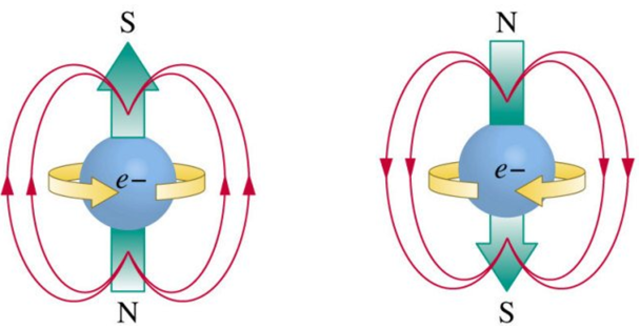
\includegraphics[width=0.5\linewidth]{imagens/spin.png}
\caption*{Fonte: Wikimedia Commons, disponível em https://shorturl.at/jEFL2}
\end{figure}

Conforme pode ser observado na Figura \ref{fig:spin}, o movimento de rotação do elétron (indicado pela seta circular de cor amarela na posição central de cada elétron) tem como consequência a geração de um \textbf{campo magnético} em cada elétron. Uma vez que os movimentos de rotação são opostos, os campos magnéticos gerados também são opostos entre si e isso os atrai. Não há como inserir um terceiro elétron em cada orbital por causa da repulsão que seria gerada por um ou outro elétron já existente no dado orbital.

\section{O conceito de hibridização}
Uma ligação química do tipo \textbf{covalente} é formada pelo compartilhamento de ao menos um elétron de um átomo com outro átomo. Para formar essa ligação, é necessário que um átomo possua um orbital semi-preenchido (com apenas um elétron) em seu subnível mais energético. A Figura \ref{fig:hibridacao_traduzida} mostra, na primeira linha, os subníveis do átomo de carbono e como seus elétrons distribuem-se nos subníveis. Repare que o subnível 2p possui três orbitais e apenas dois destes estão semi-preenchidos. Assim, o carbono forma apenas 2 ligações covalentes, contrariando o conhecimento secular estabelecido por Kekulé.

Como explicar a tetravalência do átomo de Carbono (capacidade de formar 4 ligações químicas)? Precisamos encontrar uma solução para obter um conjunto de \textbf{quatro orbitais semi-preenchidos}, mas o modo como a distribuição eletrônica do Carbono se apresenta não permite a existência dos quatro orbitais semi-preenchidos. Existe uma outra variável nesse problema: o mais simples dos hidrocarbonetos, chamado \textbf{metano} e com fórmula \textbf{\ce{CH4}}, possui 4 ligações covalentes simples e todas são quimicamente equivalentes, conforme pode ser visto na Figura \ref{fig:metanodetalhado}, ao lado direito. Nosso problema relacionado com as ligações químicas no átomo de Carbono aumentou.

\begin{figure}[H]
	\centering
	\caption{Detalhes estuturais do hidoarboneto chamado \textbf{metano} (\ce{CH4})}
	\vspace{0.5cm}
	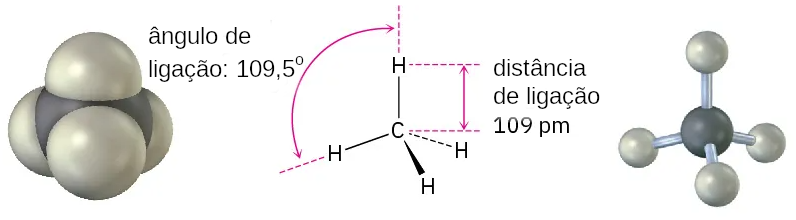
\includegraphics[width=0.8\linewidth]{imagens/metano_detalhado.png}
	\label{fig:metanodetalhado}
	\caption*{Fonte: LibreTexts (adaptada), disponível em https://shorturl.at/nzLTX}
\end{figure}

Esse problema, e sua solução, é muito importante na Química Orgânica e usaremos uma figura com linguagem visual diferente para deixar o conceito de \textbf{hibridização} o mais claro possível. 

\begin{figure}[H]
	\centering
	\caption{Esquema visual da formação de orbitais híbridos do átomo de Carbono}
	\vspace{0.5cm}
	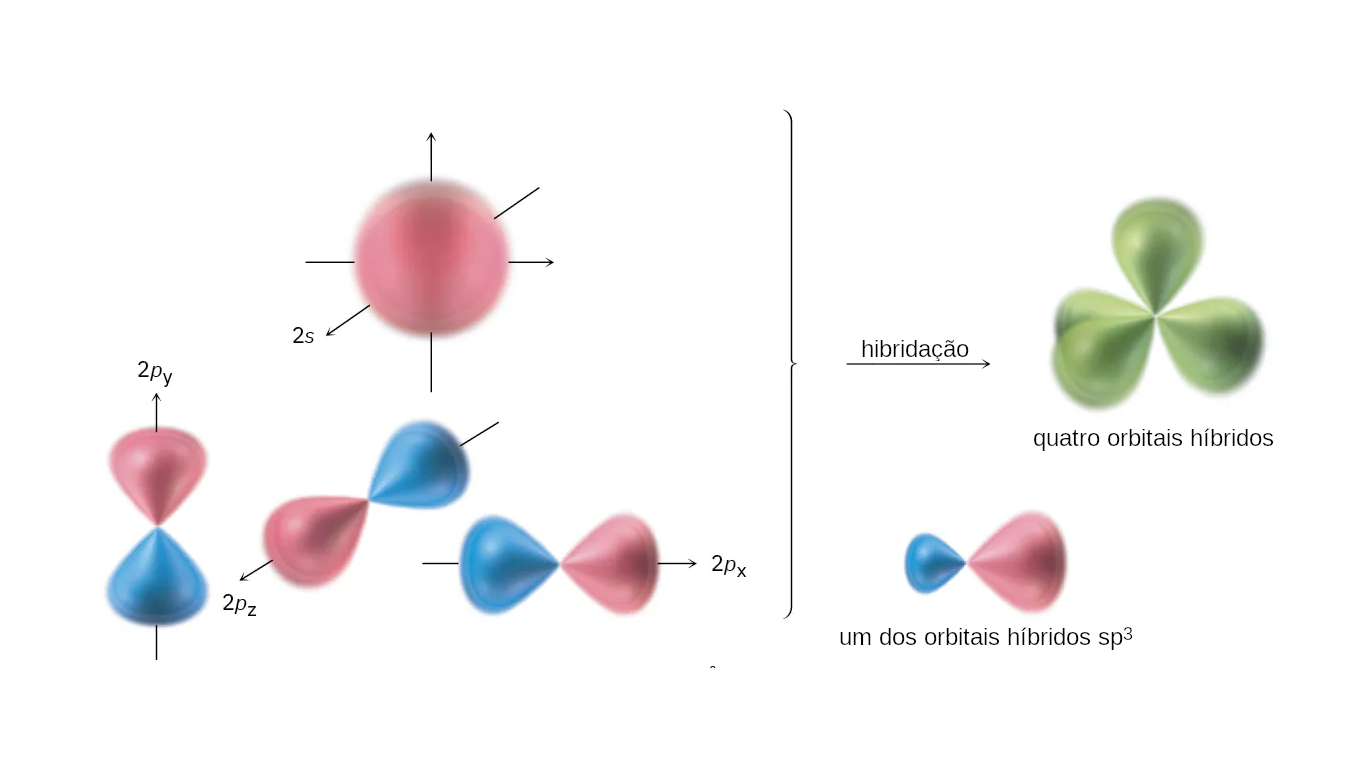
\includegraphics[width=1\linewidth]{imagens/hibridacao_visual_traduzida.png}
	\label{fig:hvt}
	\caption*{Fonte: LibreTexts (adaptada), disponível em https://shorturl.at/nzLTX}
\end{figure}

O mecanismo envolvido neste processo passa por uma combinação linear de orbitais \textbf{puros} \footnote{Usamos aqui a expressão \textbf{puro} para indicar um orbital não combinado} para formar orbitais \textbf{híbridos}, cuja composição e forma depende de quantos e quais orbitais puros foram combinados. Proposto por Linus Pauling em 1931 \cite{pauling}, o mecanismo chamado hibridização permite a existência de orbitais híbridos iguais que formam as quatro ligações químicas equivalentes no metano.

\begin{figure}[h]
\centering
\caption{Promoção eletrônica no átomo de Carbono}
\vspace{0.25cm}
\label{fig:fundexcit}
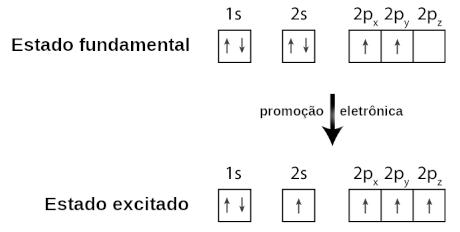
\includegraphics[width=0.7\linewidth]{imagens/fund_excit.png}
\caption*{Fonte: Wikimedia Commons (adaptada), disponível em https://shorturl.at/xyQX8}
\end{figure}

Analisando a Figura \ref{fig:fundexcit}, observamos o ponto central do processo de hibridização: a formação de orbitais \textbf{degenerados} (com mesmo conteúdo energético) através da promoção eletrônica e combinação linear dos subníveis 2s e 2p no átomo de Carbono. Uma configuração eletrônica chamada de \textbf{fundamental} é aquela que segue estritamente o \textbf{Princípio de Aufbau} ("construção", traduzido do idioma alemão e usado para a obtenção das configuraçoes eletrônicas de átomos) \cite{aufbau}; aquela que difere de algum modo da configuração do estado fundamenal é chamada de configuração \textbf{excitada}.

\begin{figure}[h]
\centering
\caption{Formação de orbitais híbridos no átomo de carbono}
\vspace{0.25cm}
\label{fig:hibridacao_traduzida}
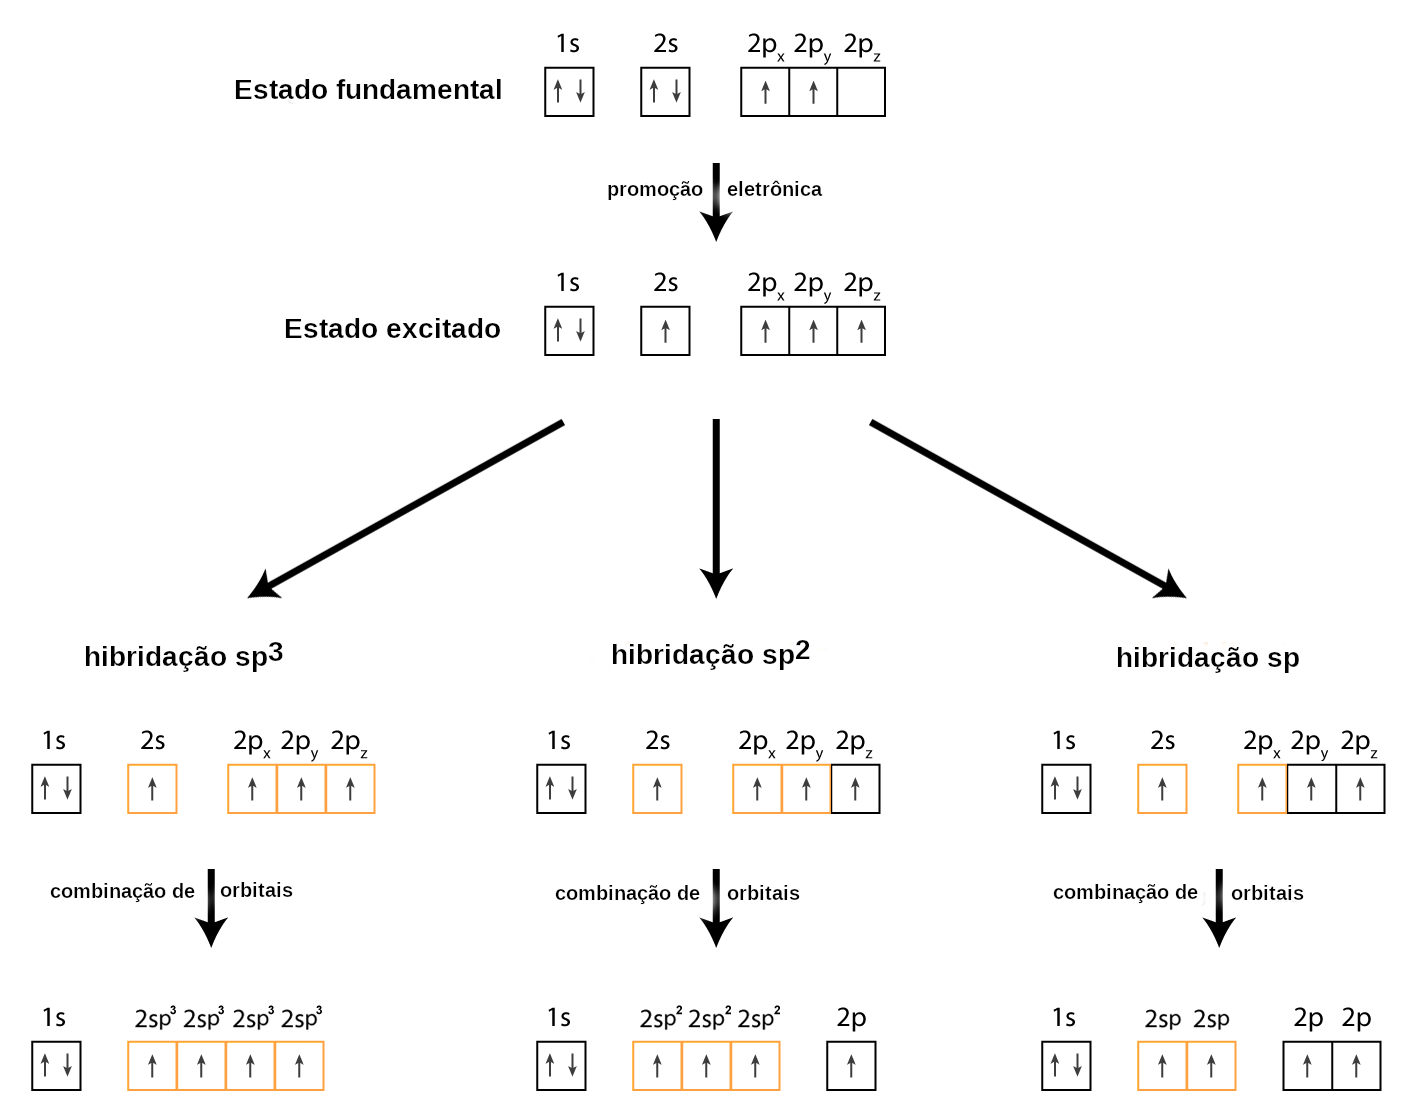
\includegraphics[width=1\linewidth]{imagens/Hybridization_of_carbon.png}
\caption*{Fonte: Wikimedia Commons (adaptada), disponível em https://shorturl.at/xyQX8}
\end{figure}

A partir da formação dos orbitais degenerados é possível, matematicamente, a existência de três combinações possíveis:

\begin{description}
	\item[\textbf{sp:}] o subnível 2s (contendo apenas um orbital) combina-se com apenas \textbf{um} dos orbitais p, restando dois orbitais puros e formando um conjunto de \textbf{dois orbitais híbridos sp}, separados entre si por 180\textcelsius.
	\item[\textbf{sp2:}] o subnível 2s (contendo apenas um orbital) combina-se com apenas \textbf{dois} dos orbitais p, restando um orbital puro e formando um conjunto de \textbf{três orbitais híbridos sp$^2$}, separados entre si por 120\textcelsius.
	\item[\textbf{sp3:}] o subnível 2s (contendo apenas um orbital) combina-se com todos os orbitais p, formando um conjunto de \textbf{quatro orbitais híbridos sp$^3$}, separados entre si por 109,5\textcelsius.
\end{description}

Os orbitais híbridos formados apresentam um arranjo espacial que justifica, em parte, a forma geométrica moléculas. A reatividade de uma molécula é explicada, em parte, por seu ambiente eletrônico, e o arranjo espacial de átomos contribui diretamente para a reatividade de substâncias orgânicas.

\section{A ligação sigma ($\sigma$)}

Uma ligação química, seja iônica ou covalente, pode ser considerada como o equilíbrio entre forças atrativas e repulsivas, conforme pode ser observado na Figura \ref{fig:dar}.

\begin{figure}[H]
	\centering
	\caption{Diagrama Lennard-Jones \cite{Lennard-Jones_1931} de forças atrativas e respulsivas na formação da molécula de H$_2$; válido para as demais ligaçãoes covalentes, respeitando a natureza de cada átomo. Observe que 1 pm = 10$^{-12}$ m}
	\vspace{0.5cm}
	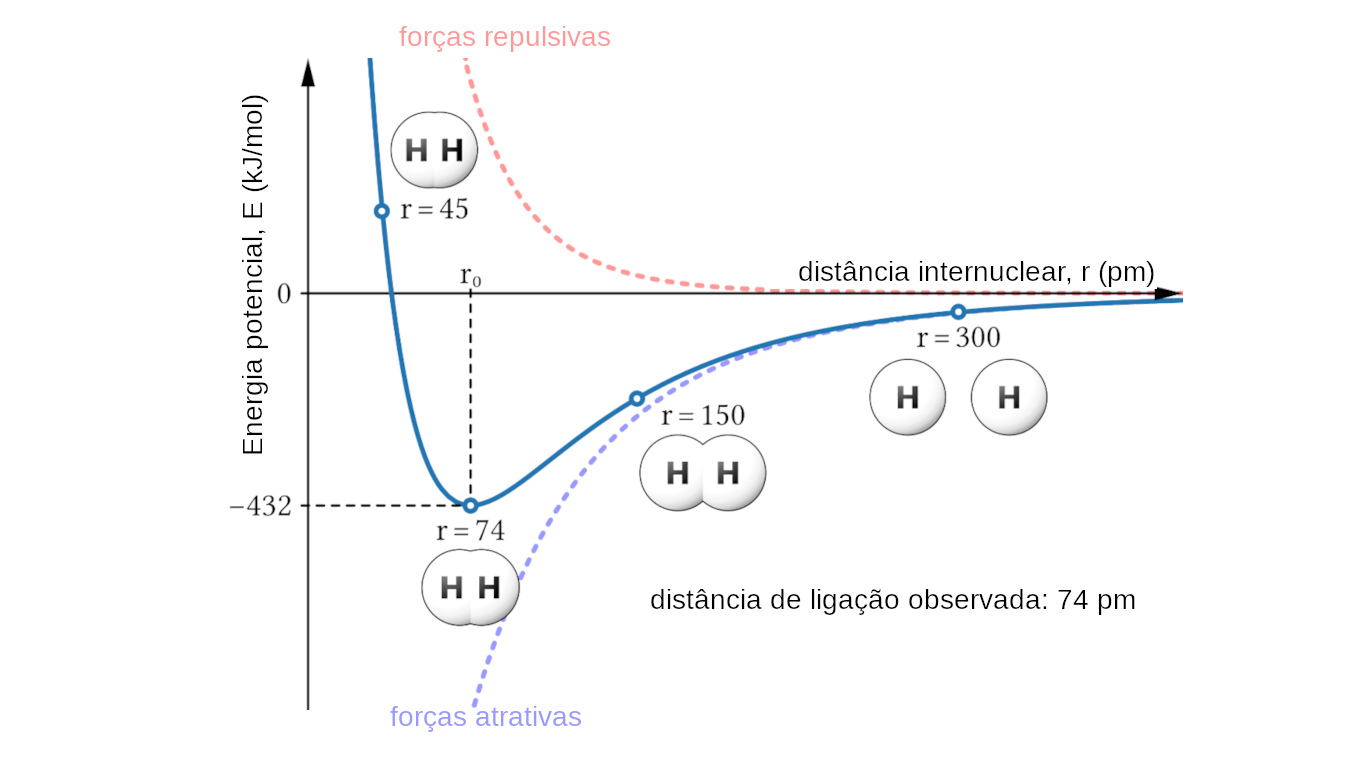
\includegraphics[width=1\linewidth]{imagens/dar.png}
	\label{fig:dar}
	\caption*{Fonte: Wikipedia (adaptada), disponível em https://shorturl.at/jDIL5}
\end{figure}

Precisamos analisar quatro regiões distintas no diagrama da Figura \ref{fig:dar}:

\begin{description}
	\item[300 pm:] nessa distância, a sobreposição dos orbitais atômicos de cada um dos átomos de Hidrogênio é praticamente nula e a estabilização que a ligação covalente traz aos átomos ainda não ocorreu. Nenhumas das forças, atrativa ou repulsiva, se manifesta a esta distância.
	\item[150 pm:] a essa distância a sobreposição dos orbitais dos átomos de Hidrogênio já ocorre em grande extensão e observa-se a predominância das forças \textbf{atrativas}, como pode ser observado pelo valor de energia negativa. 
	\item[74 pm:] nesse ponto tem-se a máxima sobreposição possível sem que perceba-se de algum componente repulsivo no sistema. A distância na qual ocorre essa sobreposição é chamada de \textbf{distância de ligação} e varia de acordo com os átomos envolvidos. 
	\item[45 pm:] em distâncias menores que 74 pm, os componentes de um dos átomos estão muito próximos daqueles do outro átomo e as forças repulsivas tornam-se muito maiores que as forças atrativas e o sistemas se desestabiliza completamente.  
\end{description}

Podemos, agora, tratar de ligações covalentes usando os conceitos de hibridização e orbitais moleculares. Uma ligação covalente do tipo $\sigma$ é aquela formada por meio da \textbf{sopreposição frontal de orbitais}, sejam puros ou híbridos. A Figura \ref{fig:sigma} apresenta à esquerda (a) uma representação que pode ser usada para compreensão do processo de formação da molécula do hidrocarboneto chamado \textbf{etano}, no qual as bolas azuis representam os átomos de Hidrogênio e o átomo de Carbono já se apresenta com seus quatro orbitais híbridos do tipo sp$^3$ em cor laranja.

O lado (b) da figura \ref{fig:sigma} mostra a molécula produzida a partir da sobreposição frontal de orbitais \textbf{s} puros dos átomos de Hidrogênio pelos orbitais híbridos \textbf{sp$^3$} dos átomos de Carbono, bem como a sobreposição frontal de orbitais híbridos de dois átomos de carbono distintos.

\begin{figure}[h]
\centering
\caption{Esquema simplificado de uma ligação $\sigma$, também chamada de ligação covalente simples.}
\vspace{0.25cm}
\label{fig:sigma}
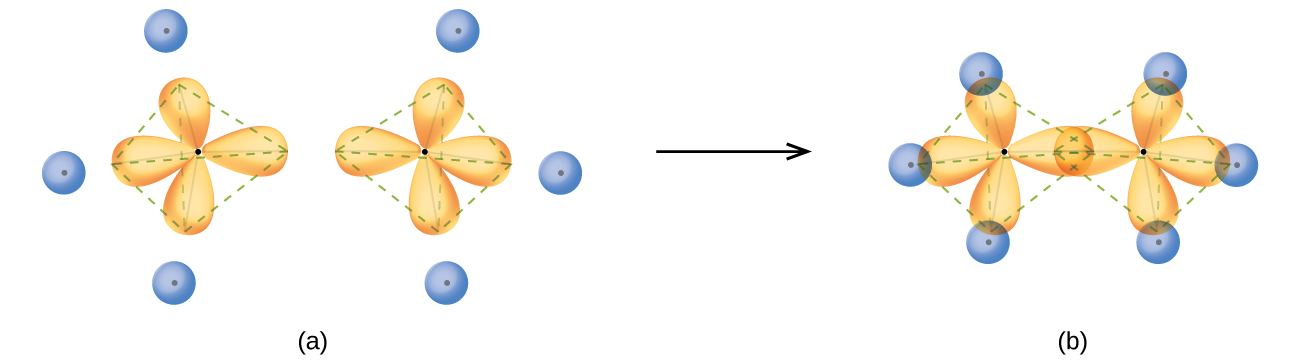
\includegraphics[width=1\linewidth]{imagens/sigma.jpg}
\caption*{Fonte: LabXchange, disponível em https://shorturl.at/zEVY6}
\end{figure}

A ligação $\sigma$ possui duas características importantes: \textbf{rotação} e \textbf{conformação}. Para exemplificar o conceito de rotação, usaremos o diagrama apresentado na Figura \ref{fig:om}.

\begin{figure}[h]
\centering
\caption{Exemplo de rotação da ligação sigma}
\vspace{0.25cm}
\label{fig:om}
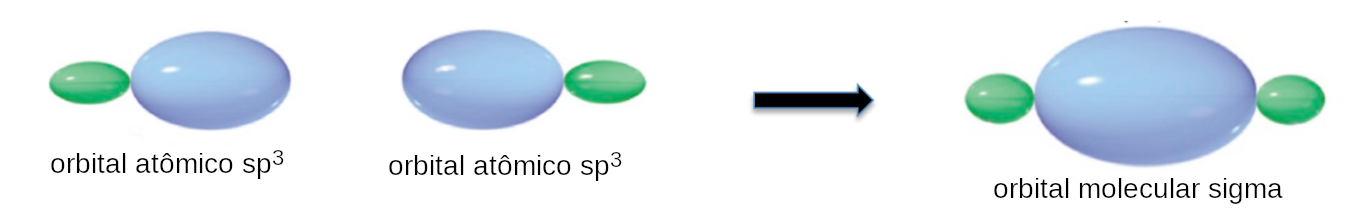
\includegraphics[width=1\linewidth]{imagens/om2.png}
\caption*{Fonte: Autores}
\end{figure}

Nosso foco está na parte \textbf{direita} da figura, onde vemos o orbital molecular formado pela sobreposição frontal de dois orbitais híbridos sp$^3$, também conhecido por ligação sigma. O ponto central da ligação que permite a rotação é a densidade eletrônica, representada pela área oval no centro imagem do lado direito da Figura \ref{fig:om} (em cor azul), estar \textbf{orientada ao longo do eixo de ligação}. O resultado final é parecido com uma barra metálica conectada a duas articulações independentes: a rotação em torno do eixo é livre. 

Com isso, podemos analisar a imagem presente na Figura \ref{fig:rotacao} para compreender como o conceito de rotação se aplica em Química Orgânica.

\begin{figure}[h]
\centering
\caption{Exemplo da rotação possível na ligação sigma ($\sigma$).}
\vspace{0.25cm}
\label{fig:rotacao}
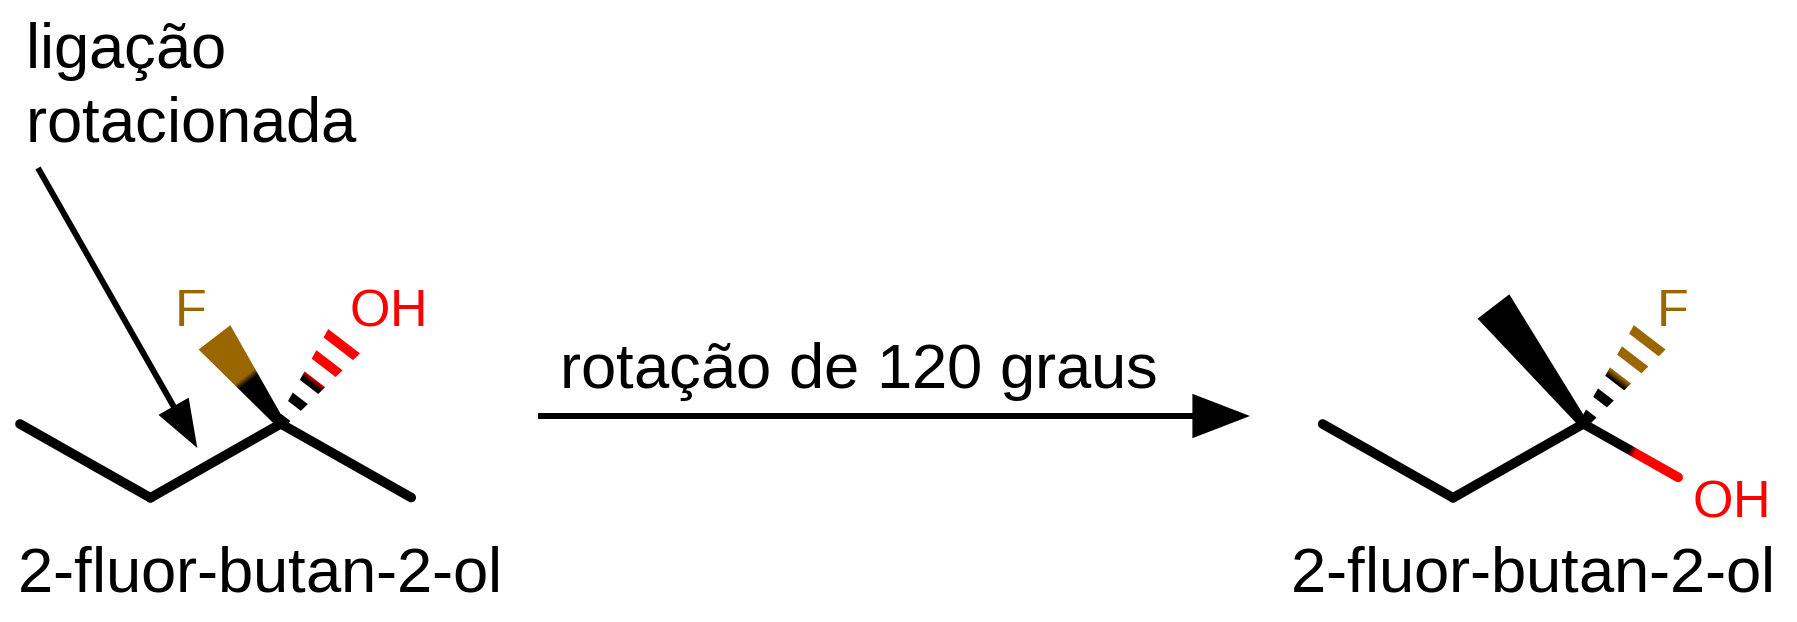
\includegraphics[width=0.75\linewidth]{imagens/rotacao.png}
\caption*{Fonte: Autores}
\end{figure}

A rotação aplicada à molécula representada à esquerda da Figura \ref{fig:rotacao} é completamente arbitrária, escolhida apernas para mostrar a liberdade rotacional presente na ligação Carbono-Carbono do tipo $\sigma$. Essa alteração rotacional ocorre muito rapidamente e modelos de dinâmica molecular podem ajudar os leitores mais curiosos \cite{Monticelli2013}. Porém, nem toda ligação sigma pode rotacionar livremente, pois ela pode fazer parte de uma cadeia cíclica ou estar associada a uma ligação $\pi$, formada pela \textbf{sobreposição lateral de orbitais puros}.

Inicialmente, considere o exemplo clássico do hidrocarboneto chamado \textbf{ciclo-hexano}, com estrutura exibida na Figura \ref{fig:ch}.

\begin{figure}[h]
\centering
\caption{Ciclo-hexano em modo bola/bastão, colorido.}
\vspace{0.25cm}
\label{fig:ch}
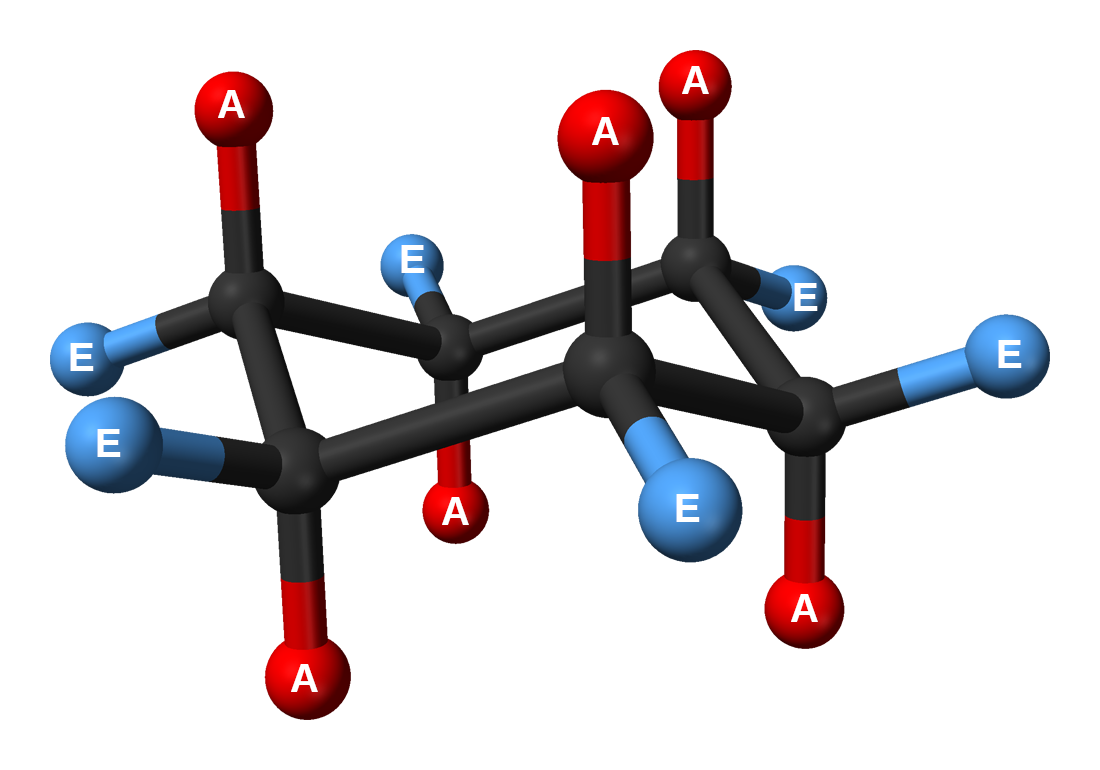
\includegraphics[width=0.6\linewidth]{imagens/Cyclohexane-chair-colour-coded-3D-balls.png}
\caption*{Fonte: Wikipedia, disponível em https://shorturl.at/fhEKU}
\end{figure}

A representação do ciclo-hexano na figura usa a notação \textbf{bola/bastão}, onde cada bastão representa uma ligação $\sigma$ (neste exemplo) e cada bola representa um átomo. Os átomos sem qualquer letra indicando símbolo são o átomos de carbono. A figura mostra dois tipos de átomos de hidrogênio nesta estrutura: aqueles marcados com a letra "A" e aqueles marcados com a letra "E". Neste exemplo, o código "A" indica os átomos de Hidrogênio em posição \textbf{axial} (considere um eixo vertical) enquanto o código "E" indica os áomos de Hidrogênio em posição \textbf{equatorial} (considere uma imaginária Linha do Equador, que divide o planeta Terra em hemisférios).

A limitada rotação possível de cada uma das ligações $\sigma$ nessa molécula causa apenas contorção e o ciclo-hexano assume diferentes \textbf{conformações}, que são arranjos espaciais provocados por rotação conjunta das ligações $\sigma$, mas limitadas em função da existência da cadeia cíclica \footnote{Não confunda \textbf{conformação} com \textbf{configuração}, pois esta última relaciona a topologia ou ordem a de conexão entre os átomos.}, conforme ilustra a figura \ref{fig:ch2}

\begin{figure}[h]
\centering
\caption{Análise conformacional do ciclo-hexano}
\vspace{0.25cm}
\label{fig:ch2}
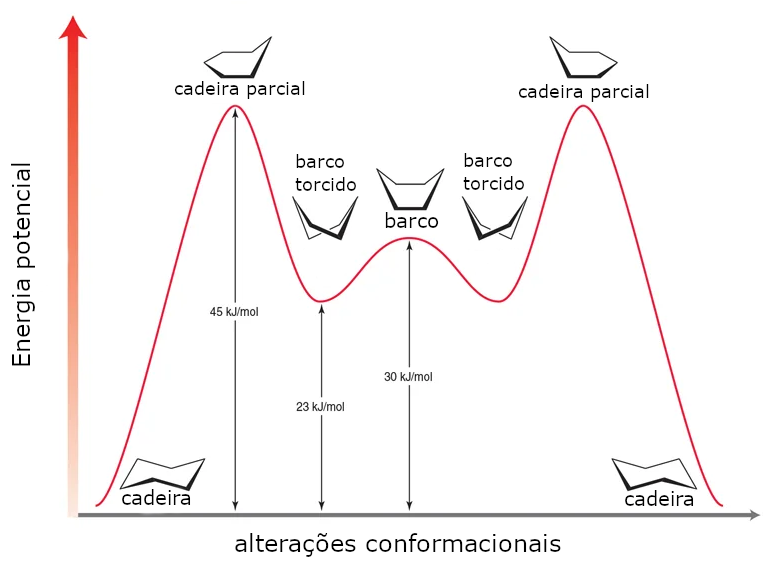
\includegraphics[width=0.85\linewidth]{imagens/analise_conformacional_ch_2.png}
\caption*{Fonte: Autores (checar origem da imagem)}
\end{figure}

A ideia central por trás dessas alterações conformacionais provocadas por rotação parcial das ligações sigma ($\sigma$) é \textbf{minimizar a repulsão eletrônica gerada por átomos de Hidrogênio}. Analisando a Figura \ref{fig:ch} podemos perceber que o ciclo-hexano em conformação \textbf{cadeira} possui energia potencial praticamente nula. Isso ocorre porque os átomos de Hidrogênio \textbf{axiais} e \textbf{equatoriais} estão distantes entre si o suficiente para eliminar uma eventual tensão angular ou torcional, estas provocadas por rotação parcial das ligações $\sigma$ entre átomos de Carbono.

A tensão que qualquer molécula pode apresentar corresponde a um excesso de energia provocado, por exemplo, por algum fator externo capaz de alterar seu estado de menor energia. Veja o caso da conformação \textbf{cadeira} do ciclo-hexano. A conformação \textbf{cadeira} possui esse nome porque existe uma certa senelhança entre a forma do ciclo-hexano nesta conformação quando comparada a uma cadeira. Você se acostuma com a ideia, acredite!

\begin{figure}[h]
\centering
\caption{Analogia da configuração cadeira do ciclo-hexano com uma cadeira.}
\vspace{0.25cm}
\label{fig:cadeira}
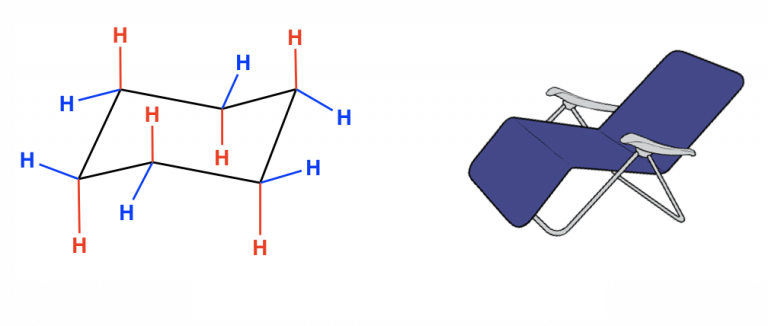
\includegraphics[width=0.75\linewidth]{imagens/chair-confirmation-analogue-768x326.png}
\caption*{Fonte: Kwantlen Polytechnic University (adaptada), disponível em https://shorturl.at/blT05}
\end{figure}

Energia fluindo do ambiente para as moléculas do ciclo-hexano a fazem vibrar e, consequentemente, torcer. Isso aumenta a repulsão entre os átomos de Hidrogênio, que era mínima, e sofre tensão torcional. Porém, um certo número de moléculas à temperatura ambiente possui energia suficiente para vibrar e, consequentemente, permitir a rotação parcial das ligações $\sigma$. Assim ocorrem as mudanças conformacionais, passando de \textbf{cadeira} para \textbf{cadeira parcial}, depois para \textbf{barco torcido}, passando para \textbf{barco}, novamente a \textbf{barco torcido} e finalmente retornando à conformação \textbf{cadeira}. A maior barreira energética para a interconversão conformacional do ciclo-hexano é de 45 kJ/mol, o que permite, à temperatura ambiente, perto de 10$^6$ conversões por segundo. Trataremos a análise conformacional em mais detalhes quando analisarmos hidrocarbonetos cíclicos.

\section{A ligação pi ($\pi$)}
Nosso cenário a respeito de ligaçãoes C-C fica um pouco mais complexo porque temos agora outro tipo de sobreposição de orbitais: a \textbf{sobreposição lateral}. Mas qual a razão deste novo tipo de sobreposição de orbitais? A frontal é insuficiente? Para compreender totalmente o novo modo de ligação que veremos a partir deste ponto, sugerimos que seja revista a Figura \ref{fig:hibridacao_traduzida}. Reproduzimos aqui uma parte da figura, destacando um ponto de grande importância na hibridização: a \textbf{combinação parcial de orbitais atômicos}.

\begin{figure}[h]
\centering
\caption{Exemplo da combinação parcial de orbitais atômicos}
\vspace{0.25cm}
\label{fig:}
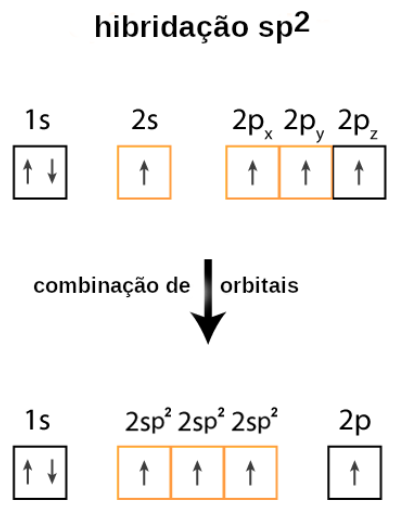
\includegraphics[width=0.45\linewidth]{imagens/sp2.png}
\caption*{Fonte: Autores}
\end{figure}

Quando o subnível 2s e o subnível 2p do átomo de Carbono tornam-se \textbf{degenerados} (igual conteúdo de energia), existem três possibilidades de combinação de orbitais puros para formar orbitais híbridos:

\begin{itemize}
	\item sp$^3$: combinação \textbf{total} entre os subníveis s e p;
	\item sp$^2$: combinação \textbf{parcial} entre os subníveis: 2s + 2 orbitais do subnível 2p;
	\item sp: combinação \textbf{parcial} entre os subníveis: 2s + 1 orbital 2p.
\end{itemize}

Nosso foco está nas combinações \textbf{parciais}, nas quais um ou dois orbitais p puros do subnível 2p não participaram do processo de combinação. Conforme podemos observar na Figura \ref{fig:vistas_sp2}, quando a combinação de orbitais envolve apenas dois dos três orbitais do subnível p, forma-se um subnível híbrido  \textbf{sp$^2$}, contendo três orbitais e um orbital p permanece intacto. Aqui está o ponto central: os três orbitais híbridos sp$^2$ são \textbf{coplanares} e o orbital p puro está em posição \textbf{ortogonal} em relação aos híbridos sp$^2$. Assim, quando dois orbitais sp$^2$ sobrepõem-se de modo frontal, formando uma ligação sigma, dois orbitais p puros ficam paralelos entre si, possibilitando a \textbf{sobreposição lateral}.

\begin{figure}[h]
\centering
\caption{Vistas lateral e superior do subnível sp$^2$}
\vspace{0.25cm}
\label{fig:vistas_sp2}
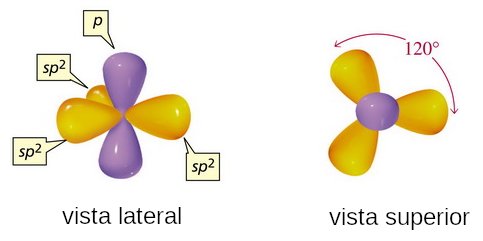
\includegraphics[width=0.65\linewidth]{imagens/hibrido_sp2.png}
\caption*{Fonte: Autores (checar a origem)}
\end{figure}

Embora a sobreposição lateral também seja uma ligação química, sua formação e propriedades são bem distintas daquela da ligação sigma, e possibilita a ocorrência de, por exemplo, duas entidades de crucial importância em Química Orgânica: \textbf{conjugação} e \textbf{ressonância}. A Figura \ref{fig:sobre_lateral} ilustra o processo de formação da ligação pi ($\pi$) por meio da sobreposição lateral de orbitais puros.

\begin{figure}[h]
\centering
\caption{Sobreposição lateral e formação da ligação $\pi$}
\vspace{0.25cm}
\label{fig:sobre_lateral}
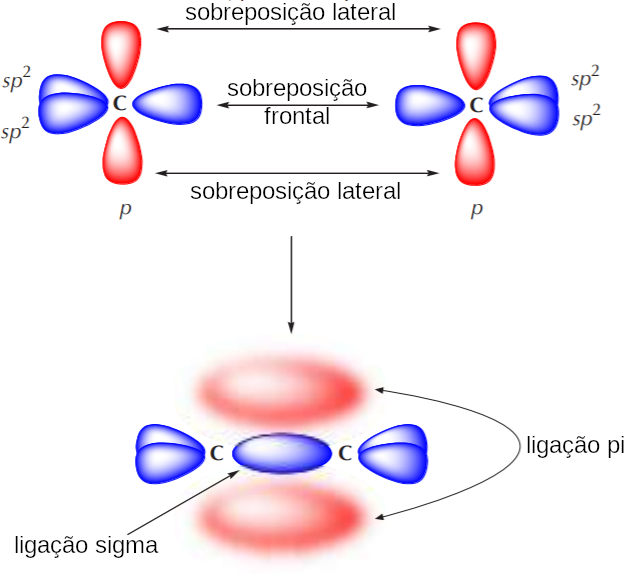
\includegraphics[width=0.75\linewidth]{imagens/sobre_lateral.png}
\caption*{Fonte: LibreTexts Chemistry (adaptada), disponível em https://shorturl.at/jnKU1}
\end{figure}

Analisando a figura \ref{fig:sobre_lateral}, percebemos o mecanismo de formação da ligação $\pi$ com a aproximação horizontal dos dois átomos de Carbono que se ligarão. Na parte superior da figura, dois orbitais híbridos se aproximam de modo horizontal e ocorrerá a sobreposição \textbf{frontal} destes orbitais, formando a ligação sigma. Porém, aproximando os dos dois átomos de Carbono também aproximam-se dois orbitais \textbf{p} puros o suficiente para que ocorra a \textbf{sobreposição lateral} destes orbitais.

Como o orbital p puro é formado por dois lobos, um acima e outro abaixo do plano nodal (aquele que passa pelo núcleo do átomo), existem duas regiões de sobreposição, uma acima e outra abaixo da ligação $\sigma$. Considerando que orbitais estão diretamente relacionados com probabilidade de encontrar um elétron, de forma muito simplificada, podemos encontrar o par eletrônico da ligação $\pi$ \textbf{acima} ou \textbf{abaixo} da ligação $\sigma$, o que justifica as duas regiões presentes na parte de baixo da Figura \ref{fig:sobre_lateral}.

Existem outras possibilidades de combinação entre os orbitais, como por exemplo aquela que envolve um orbital puro \textbf{s} e um orbital puro \textbf{p}, formando um conjunto de orbitais híbridos chamado de \textbf{sp}, característicos de ligações carbono-carbono do tipo tripla (\ce{-C#C-}) ou então de sistemas \textbf{alênicos}, onde temos três átomos de carbono ligados por \textbf{duas} ligações duplas (\ce{C=C=C}).

No caso da ligação carbono-carbono do tipo tripla, os dois átomos de carbono apresentam hibridização sp e geometria linear, assim como o carbono central do sistema alênico, o que confere algumas características químicas partculares a sistemas como os descritos, conforma pode ser visto na figura \ref{fig:tripla}.

\begin{figure}[h]
\centering
\caption{Carbonos com hibridização sp: a ligação tripla}
\vspace{0.25cm}
\label{fig:tripla}
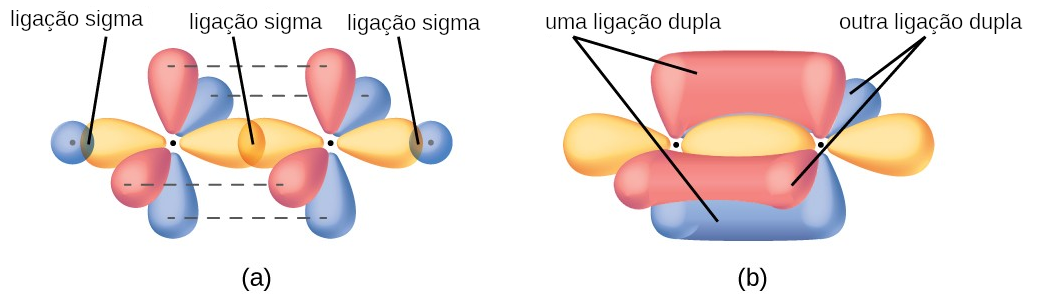
\includegraphics[width=1\linewidth]{imagens/tripla.png}
\caption*{Fonte: LibreTexts, adaptada, disponível em https://shorturl.at/hikBG}
\end{figure}

Analisando a parte (a) da figura \ref{fig:tripla}, percebemos a sobreposição frontal de orbitais puros ou híbridos (ligação $\sigma$) e também um tracejado que indica a sobreposição lateral de orbitais p puros (ligação $\pi$). Ao analisarmos a parte (b) da mesma figura, identificamos, com cores diferentes, as duas ligações duplas formadas entre dois átomos de carbono com hibridização sp. 